\documentclass[conference]{IEEEtran}

\usepackage{cite}
\usepackage{amsmath,amssymb}
\usepackage{graphicx}
\usepackage{booktabs}
\usepackage{array}
\usepackage{url}
\usepackage[hidelinks]{hyperref}
\usepackage{microtype}
\usepackage{multirow}
\usepackage{balance}

\graphicspath{{figures/}}

\title{An Error-Sensitive and Reproducible Baseline for SMS Spam Detection Using Bag-of-Words and Multinomial Naive Bayes}

\author{
\IEEEauthorblockN{Aritrik Ghosh}
\IEEEauthorblockA{
Department of Computer Science and Engineering\\
Swami Vivekananda University, India}
}

\begin{document}
\maketitle

\begin{abstract}
SMS spam detection is a compact but practical natural-language processing problem in which legitimate and unwanted messages must be distinguished from short, noisy, and highly variable text. This paper evaluates a deliberately lightweight detection pipeline based on word-count features and Multinomial Naive Bayes, while extending the evaluation beyond headline accuracy to provide an error-sensitive view of operational behavior and reproducibility. The experiment uses a 5,559-message CSV derived from the public SMS Spam Collection, with 4,812 legitimate messages and 747 spam messages. An 80\%--20\% hold-out split with a fixed random seed is used, and CountVectorizer is fitted only on the training partition. On the held-out test set, the proposed baseline obtains 99.01\% accuracy, 100\% spam precision, 91.73\% spam recall, and 95.69\% spam F1-score. The confusion matrix contains 979 true negatives, 122 true positives, 11 false negatives, and zero false positives. From these observations, the balanced accuracy is 95.86\%, the false-negative rate is 8.27\%, and the Matthews correlation coefficient is 0.9524. The paper's contribution is intentionally methodological rather than algorithmic: it combines dataset-provenance transparency, leakage-safe feature construction, error-sensitive reporting, and a reproducible lightweight implementation into a single baseline. This framing is useful because high aggregate accuracy can obscure practically important error asymmetry in imbalanced SMS data. The resulting system is not presented as state of the art, nor is measured resource efficiency claimed; instead, it is positioned as a transparent and reproducible baseline for student research and reproducibility-oriented studies.
\end{abstract}

\begin{IEEEkeywords}
SMS spam detection, text classification, bag-of-words, CountVectorizer, Multinomial Naive Bayes, imbalanced classification, error analysis, reproducibility
\end{IEEEkeywords}

\section{Introduction}
Mobile messaging is a communication channel in which unwanted commercial, fraudulent, and phishing-oriented content can reach users directly. Automatic SMS filtering is therefore a small but meaningful application of natural language processing (NLP) and cybersecurity. Compared with long-form document classification, SMS classification must operate on short messages that can contain abbreviations, spelling variation, punctuation, URLs, numbers, and intentionally unusual wording. Earlier studies of mobile spam filtering emphasized that these properties affect both representation and classifier design~\cite{cormack2007feature,cormack2007spam}.

The availability of public SMS corpora has made the problem attractive for reproducible machine-learning research. Almeida, Hidalgo, and Yamakami introduced a public SMS spam corpus and evaluated several established learning methods, addressing a major obstacle in the area: the scarcity of publicly accessible datasets suitable for controlled comparison~\cite{almeida2011sms}. The same collection is now catalogued by the UCI Machine Learning Repository~\cite{uci_sms}.

Classical supervised learning remains relevant despite the growth of neural and transformer-based text models. Bag-of-words representations are simple, sparse, interpretable, and inexpensive to compute, while Multinomial Naive Bayes is specifically suited to discrete count-like text features~\cite{mccallum1998nb}. For short-message filtering, such a model provides an attractive baseline because it can be trained on an ordinary CPU and inspected without specialized infrastructure.

However, a common weakness of small classification studies is an overemphasis on a single aggregate metric. In imbalanced binary classification, accuracy can be high even when the minority class is not detected reliably. Precision-recall analysis has therefore been recommended as an especially informative perspective when classes are skewed~\cite{davis2006pr,saito2015pr}. For an SMS filter, the practical meaning of a false positive and a false negative is different: incorrectly rejecting a legitimate message is not operationally equivalent to allowing one spam message through.

This paper therefore addresses the following research questions.

\textbf{RQ1:} How accurately can a lightweight CountVectorizer--Multinomial Naive Bayes pipeline classify the supplied SMS corpus?

\textbf{RQ2:} What does the confusion matrix reveal about the balance between missed spam and incorrectly flagged legitimate messages?

\textbf{RQ3:} Can dataset provenance, leakage-safe preprocessing, and error-sensitive metrics provide a more reproducible and informative baseline than reporting accuracy alone?

The paper does not claim a new learning algorithm. Its methodological contribution is an integrated, auditable evaluation pattern for a student-scale study: (i) explicit distinction between the official public corpus and the exact local CSV used in the experiment; (ii) strict training-only vocabulary fitting; (iii) error-sensitive analysis using derived measures in addition to accuracy; and (iv) a reproducible implementation based on widely used external scientific Python packages. Resource use is discussed qualitatively because runtime, memory, and throughput were not recorded in the original experiment. The result is positioned as a transparent baseline that can be extended to stronger classifiers and newer datasets.

The remainder of the paper reviews the literature, defines the experimental design, explains implementation details, reports the observed results, analyzes the operational error profile, and discusses the scope and limits of the findings.

\section{Related Work}
\subsection{Classical Text Categorization}
Automated text categorization has a long history in information retrieval and machine learning. Sebastiani's survey organized the field around document representation, classifier construction, and evaluation, emphasizing that these components are interdependent rather than interchangeable~\cite{sebastiani2002ml}. Earlier term-weighting work by Salton and Buckley established the importance of representation choices in text retrieval and provides the conceptual background for sparse lexical features~\cite{salton1988term}.

Naive Bayes is particularly attractive for sparse text. McCallum and Nigam compared Bernoulli and multinomial event models and reported that the multinomial representation can be especially effective as vocabulary size grows~\cite{mccallum1998nb}. Support Vector Machines also became an influential classical baseline for high-dimensional text because they can learn robust decision boundaries in sparse feature spaces~\cite{joachims1998svm}. These methods established an important design principle for practical NLP: sophisticated linguistic modeling is not always necessary to obtain strong classification performance.

Androutsopoulos \textit{et al.} examined statistical spam filtering using machine-learning techniques and demonstrated the usefulness of probabilistic approaches for unwanted-message detection~\cite{androutsopoulos2000spam}. Almeida, Almeida, and Yamakami later studied how dimensionality reduction affects Naive Bayes spam filtering, reinforcing the role of feature-space design in probabilistic spam models~\cite{almeida2011dim}.

\subsection{SMS-Specific Filtering}
SMS spam introduces additional challenges because messages are short and often noisy. Cormack \textit{et al.} investigated feature engineering specifically for mobile SMS spam and argued that standard e-mail filtering assumptions may require adaptation~\cite{cormack2007feature}. Their related study on short-message filtering analyzed the difficulty of classification when each example contains relatively little text~\cite{cormack2007spam}.

The SMS Spam Collection introduced by Almeida \textit{et al.} became an important public benchmark for this line of research~\cite{almeida2011sms}. Later work investigated text normalization and semantic indexing to address abbreviations, symbols, slang, and other irregularities found in short messages~\cite{almeida2016normalization}. Other research explored parsimonious or minimum-description-length ideas for spam filtering, illustrating that simplicity itself can be a meaningful design objective~\cite{almeida2012occam}.

\subsection{Recent Directions}
Recent literature shows a progression from classical sparse representations toward deep learning, semantic normalization, and more systematic comparative pipelines. A 2024 survey by Al Saidat, Yerima, and Shaalan reviewed NLP and machine-learning approaches for SMS spam and smishing detection and highlighted the increasing use of deep neural methods~\cite{saidat2024survey}. A 2026 study by Senol, Takci, and Seker systematically compared feature extraction, feature selection, class-imbalance handling, scaling, and multiple classifiers on the UCI SMS corpus, showing that relatively simple bag-of-words configurations can remain competitive while offering low computational cost~\cite{senol2026pipeline}.

These recent studies motivate a practical question for smaller research projects. When a student or practitioner has only one day, limited hardware, and a need for reproducibility, it may be more useful to understand a strong classical baseline and its error profile than to immediately reproduce a large model comparison.

\begin{table}[t]
\caption{Representative Research Directions and Their Relation to This Study}
\label{tab:related}
\centering
\scriptsize
\begin{tabular}{p{1.55cm}p{2.35cm}p{2.75cm}}
\toprule
Study & Main emphasis & Relation to present work \\
\midrule
Sebastiani~\cite{sebastiani2002ml} & General text categorization & Foundations of representation and evaluation \\
McCallum and Nigam~\cite{mccallum1998nb} & Naive Bayes event models & Statistical basis for MNB \\
Androutsopoulos \textit{et al.}~\cite{androutsopoulos2000spam} & Statistical spam filtering & Spam-classification baseline \\
Cormack \textit{et al.}~\cite{cormack2007feature} & SMS feature engineering & Short-message representation challenge \\
Cormack \textit{et al.}~\cite{cormack2007spam} & Short-message spam filtering & SMS-specific evaluation context \\
Almeida \textit{et al.}~\cite{almeida2011sms} & Public SMS corpus and classifiers & Dataset foundation \\
Almeida \textit{et al.}~\cite{almeida2016normalization} & Semantic normalization & More complex text preprocessing direction \\
Al Saidat \textit{et al.}~\cite{saidat2024survey} & Modern NLP/ML survey & Recent landscape \\
Senol \textit{et al.}~\cite{senol2026pipeline} & Systematic multi-model pipeline & Recent evidence for efficient BoW baselines \\
Present study & Error-sensitive reproducible baseline & Focus on transparency, errors, and lightweight execution \\
\bottomrule
\end{tabular}
\end{table}

\subsection{Positioning and Research Gap}
Delany, Buckley, and Greene reviewed SMS spam filtering methods and data issues, emphasizing that corpus construction and availability are central to valid comparisons~\cite{delany2012methods}. Early content-based SMS work also evaluated multiple classical classifiers on SMS collections, reinforcing the value of simple lexical baselines as reference points~\cite{gomez2006content}.

The literature suggests that SMS spam detection is not primarily constrained by the absence of classifiers; many choices already exist. The more realistic gap for a small reproducibility-oriented study is methodological: students frequently reproduce a single accuracy number without documenting dataset provenance, split policy, minority-class behavior, or the exact error distribution. This paper targets that narrower gap. It uses a conventional classifier but makes the experimental chain explicit and interprets the result through an error-sensitive lens.

Accordingly, the novelty claim is deliberately limited. The study does not introduce a new feature extractor, classifier, neural architecture, or dataset. Instead, it contributes a reproducibility-oriented evaluation pattern that is easy to audit and serves as a controlled starting point for future comparisons.

\section{Proposed Evaluation Framework}
\subsection{Research Design}
The evaluation is designed as a controlled single-model experiment. The independent design choices are the dataset version, word-count representation, and Multinomial Naive Bayes classifier. The outcome variables are accuracy, precision, recall, F1-score, confusion-matrix counts, balanced accuracy, false-positive rate, false-negative rate, negative predictive value, and Matthews correlation coefficient (MCC).

The design can be summarized as
\begin{equation}
D \rightarrow D_{train},D_{test} \rightarrow \mathrm{CountVectorizer} \rightarrow \mathrm{MNB} \rightarrow \hat{y} \rightarrow E,
\end{equation}
where $D$ denotes the supplied labeled dataset and $E$ denotes the evaluation stage.

The experiment intentionally uses a fixed random seed so that the reported test set is deterministic. This does not eliminate sampling uncertainty, but it makes the exact experiment reproducible.

\subsection{Dataset Provenance}
The local file supplied for this study is named \texttt{spamraw.csv}. It contains 5,559 usable rows with the columns \texttt{type} and \texttt{text}. Exploratory analysis reports 4,812 ham messages and 747 spam messages. The official UCI record for the SMS Spam Collection lists 5,574 instances~\cite{uci_sms}. The 15-row difference is therefore explicitly documented as a provenance difference between the public record and the local working file.

This distinction is important for reproducibility. A result obtained from a local subset should not be presented as if it were necessarily obtained from every record in the public release. The present paper therefore treats the supplied 5,559-row file as the authoritative experimental dataset.



\subsection{Train/Test Procedure}
The original experiment uses \texttt{train\_test\_split} with \texttt{test\_size=0.20} and \texttt{random\_state=0}. The split contains 4,447 training instances and 1,112 test instances. Stratification was not applied, and the present paper does not retroactively change the experiment after seeing the results.

The absence of stratification is an explicit limitation. In a follow-up study, repeated stratified splits or cross-validation would be preferable for estimating variance and making model comparisons. The confidence intervals in Table~\ref{tab:results} quantify uncertainty for the present split, but they do not replace repeated evaluation across alternative partitions. Nevertheless, documenting the original procedure is necessary if the paper is to remain faithful to the actual experiment.

\subsection{CountVectorizer Representation}
CountVectorizer maps each message to a sparse vector of token counts. Let $V=\{v_1,\dots,v_m\}$ denote the training vocabulary. A message $d$ becomes
\begin{equation}
\mathbf{x}_d=[c(v_1,d),c(v_2,d),\ldots,c(v_m,d)],
\end{equation}
where $c(v_i,d)$ is the frequency of token $v_i$ in $d$.

The vectorizer is fitted only on the training partition:
\begin{equation}
X_{train}=f_{fit}(D_{train}), \qquad X_{test}=f_{transform}(D_{test}).
\end{equation}
This ordering is important because fitting a vocabulary on the full dataset would allow information from the test partition to influence the feature construction process.

Bag-of-words does not model word order explicitly. Consequently, two messages containing the same words can receive similar representations even when their phrasing differs. For SMS data, this limitation is partly offset by the discriminative information carried by promotional vocabulary, numerical expressions, and other lexical patterns.

\subsection{Multinomial Naive Bayes Model}
The Multinomial Naive Bayes classifier estimates the posterior probability of a class $c$ given a message vector $\mathbf{x}$ according to
\begin{equation}
P(c\mid\mathbf{x})\propto P(c)\prod_{i=1}^{m}P(x_i\mid c).
\end{equation}

The naive conditional-independence assumption is not literally true for natural language, since words interact and phrases carry contextual meaning. Nevertheless, the model is attractive because parameter estimation is simple, training is fast, and the resulting classifier is well matched to sparse word-count features~\cite{mccallum1998nb}.

\subsection{Evaluation Metrics}
The primary measures are accuracy, precision, recall, and F1-score. Because binary classification on imbalanced data can make accuracy and F1 appear overly optimistic, MCC is included as a complementary summary of all four confusion-matrix cells~\cite{chicco2020mcc}. Accuracy is
\begin{equation}
Accuracy=\frac{TP+TN}{TP+TN+FP+FN}.
\end{equation}

For spam as the positive class,
\begin{equation}
Precision=\frac{TP}{TP+FP}, \qquad Recall=\frac{TP}{TP+FN},
\end{equation}
\begin{equation}
F1=2\frac{Precision\cdot Recall}{Precision+Recall}.
\end{equation}

Because the dataset is imbalanced, two additional measures are derived from the observed confusion matrix. Specificity is
\begin{equation}
Specificity=\frac{TN}{TN+FP},
\end{equation}
and the false-negative rate is
\begin{equation}
FNR=\frac{FN}{TP+FN}=1-Recall.
\end{equation}

Balanced accuracy gives equal weight to the positive and negative class recalls:
\begin{equation}
BA=\frac{Recall+Specificity}{2}.
\end{equation}

Finally, MCC is included because it summarizes all four confusion-matrix cells in a single correlation-style statistic~\cite{chicco2020mcc}:
\begin{equation}
MCC=\frac{TP\cdot TN-FP\cdot FN}{\sqrt{(TP+FP)(TP+FN)(TN+FP)(TN+FN)}}.
\end{equation}
The use of precision, recall, and related measures is particularly relevant for skewed binary classification~\cite{davis2006pr,saito2015pr}.

\section{Implementation and Reproducibility}
\subsection{Software Environment}
The implementation uses Python and external scientific machine-learning libraries. These include NumPy, pandas, matplotlib, seaborn, and scikit-learn; they are not Python standard-library modules. The core dependencies are NumPy, pandas, matplotlib, seaborn, and scikit-learn. Scikit-learn provides the train/test utilities, CountVectorizer, MultinomialNB, and evaluation functions used in the experiment~\cite{pedregosa2011sklearn}.

No GPU, distributed system, external API, or proprietary software is required by the implementation. This makes the pipeline suitable for ordinary CPU-based experimentation, but the present study does not claim a measured runtime or memory advantage because those quantities were not recorded.

\subsection{Pipeline Steps}
The implementation follows seven steps.
\begin{enumerate}
\item Read the CSV file and inspect the schema.
\item Separate the label column \texttt{type} from the message column \texttt{text}.
\item Perform a fixed 80/20 train/test split with random seed 0.
\item Fit CountVectorizer on training text and transform both partitions.
\item Train Multinomial Naive Bayes on the sparse training matrix.
\item Generate predictions for the held-out test messages.
\item Compute classification metrics and the confusion matrix.
\end{enumerate}

\begin{figure}[t]
\centering
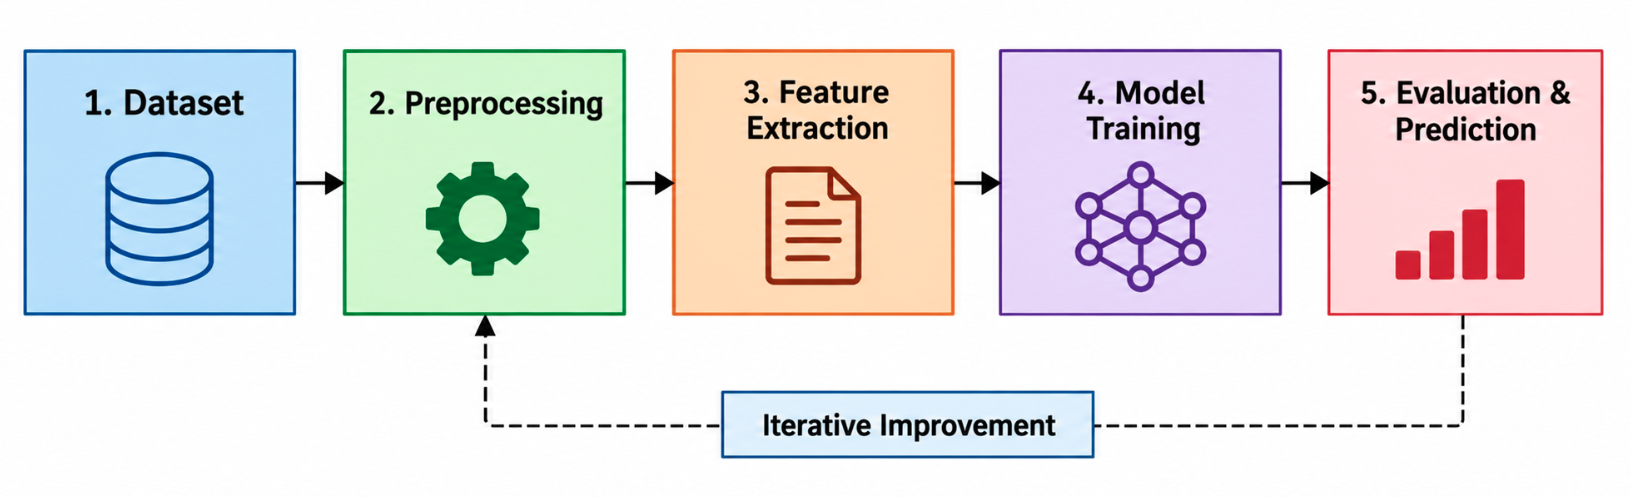
\includegraphics[width=0.96\columnwidth]{figures/architecture.png}
\caption{End-to-end architecture of the proposed lightweight SMS spam detection pipeline.}
\label{fig:architecture}
\end{figure}

Figure~\ref{fig:architecture} emphasizes the controlled separation between training and evaluation data. The most important reproducibility property is not architectural complexity, but the preservation of this boundary.

\subsection{Algorithmic Description}
The complete procedure can be summarized as follows.

\begin{table}[t]
\caption{Reproducible Experimental Configuration}
\label{tab:config}
\centering
\scriptsize
\begin{tabular}{ll}
\toprule
Parameter & Value \\
\midrule
Input file & \texttt{spamraw.csv} \\
Rows & 5,559 \\
Target column & \texttt{type} \\
Text column & \texttt{text} \\
Split & 80/20 hold-out \\
Random seed & 0 \\
Stratification & No \\
Feature method & CountVectorizer (default parameters) \\
Classifier & MultinomialNB (default parameters) \\
Primary metrics & Accuracy, precision, recall, F1 \\
Secondary metrics & BA, FPR, FNR, MCC, NPV \\
Hardware & CPU-only execution; exact machine not recorded \\
\bottomrule
\end{tabular}
\end{table}

\noindent\textbf{Algorithm 1: Reproducible SMS Spam Baseline}
\begin{enumerate}
\item Input labeled messages $D$.
\item Split $D$ into $D_{train}$ and $D_{test}$ using the recorded seed.
\item Fit the vocabulary on $D_{train}$ only.
\item Transform $D_{train}$ and $D_{test}$ into sparse count matrices.
\item Fit Multinomial Naive Bayes on the training matrix.
\item Predict the labels of $D_{test}$.
\item Compute all primary and derived metrics from the same confusion matrix.
\item Store the metrics and figures so the manuscript can be regenerated.
\end{enumerate}

\subsection{Reproducibility Controls}
The experiment follows several controls. First, the exact local dataset size is reported. Second, the train/test split is deterministic. Third, the vectorizer is trained only on the training partition. Fourth, results are derived directly from stored predictions rather than manually transcribed. Fifth, the confusion matrix is treated as the source for the secondary error metrics.

This design does not solve dataset shift or sampling uncertainty, but it reduces avoidable ambiguity. The supplied experiment did not record the exact Python, NumPy, pandas, or scikit-learn versions, nor did it archive a checksum of the local CSV. These missing artifacts are therefore identified as reproducibility limitations rather than guessed in this manuscript. In particular, it makes it possible for a second researcher to identify whether a disagreement is caused by a different dataset version, split, preprocessing sequence, or classifier configuration.

\section{Results}
\subsection{Dataset-Level Findings}
The experimental CSV contains 5,559 messages, of which 4,812 are ham and 747 are spam. The spam proportion in the full local dataset is therefore approximately 13.44\%. The held-out test set contains 133 spam messages and 979 ham messages, producing a test-set spam prevalence of approximately 11.96\%.

The difference between full-dataset prevalence and test-set prevalence is a consequence of using a non-stratified random split. This is one reason why reporting the split policy is essential when a classifier is evaluated on imbalanced data.

\subsection{Primary Performance}
Table~\ref{tab:results} reports the observed test-set metrics supplied with the experiment.

\begin{table}[t]
\caption{Observed Performance on the 1,112-Message Test Set}
\label{tab:results}
\centering
\scriptsize
\begin{tabular}{lcc}
\toprule
Metric & Value & 95\% CI \\
\midrule
Accuracy & 99.01\% & 98.24--99.45\% \\
Spam precision & 100.00\% & 96.95--100.00\% \\
Spam recall & 91.73\% & 85.80--95.32\% \\
Spam F1-score & 95.69\% & 92.91--98.01\%$^{a}$ \\
Weighted precision & 99.02\% & -- \\
Weighted recall & 99.01\% & -- \\
Weighted F1-score & 98.99\% & -- \\
Balanced accuracy & 95.86\% & -- \\
Specificity & 100.00\% & 99.61--100.00\% \\
False-positive rate & 0.00\% & -- \\
False-negative rate & 8.27\% & -- \\
Negative predictive value & 98.89\% & -- \\
MCC & 0.9524 & -- \\
\bottomrule
\end{tabular}
\vspace{1mm}
\parbox{0.96\columnwidth}{\scriptsize $^{a}$Approximate multinomial bootstrap interval from the observed four-cell confusion matrix; Wilson score intervals are used for binomial proportions.}
\end{table}

The observed accuracy is 99.01\%. For the spam class, precision is 1.00 and recall is 0.9173, resulting in an F1-score of 0.9569. The perfect spam precision on this split is caused by the absence of false positives, not by a guarantee that false positives can never occur. Because these estimates come from a single fixed partition, uncertainty should also be reported. Using 95\% Wilson score intervals for binomial proportions~\cite{agresti1998ci}, accuracy is 99.01\% (95\% CI: 98.24--99.45\%), spam precision is 100.00\% (95\% CI: 96.95--100.00\%), spam recall is 91.73\% (95\% CI: 85.80--95.32\%), and specificity is 100.00\% (95\% CI: 99.61--100.00\%). For F1, a multinomial bootstrap over the four observed confusion-matrix outcome cells gives an approximate 95\% interval of 92.91--98.01\%; this interval is a resampling diagnostic from the aggregate confusion matrix rather than a substitute for repeated experiments on the underlying messages.

The derived balanced accuracy of 95.86\% is lower than the overall accuracy because balanced accuracy gives equal importance to both class recalls. This difference illustrates why the single accuracy number should not be treated as the only summary of model behavior.

\subsection{Confusion Matrix and Error Profile}
The confusion matrix is
\begin{equation}
C=\begin{bmatrix}
979 & 0\\
11 & 122
\end{bmatrix}.
\end{equation}
Rows represent the true class and columns the predicted class, ordered as ham and spam.

\begin{figure}[t]
\centering
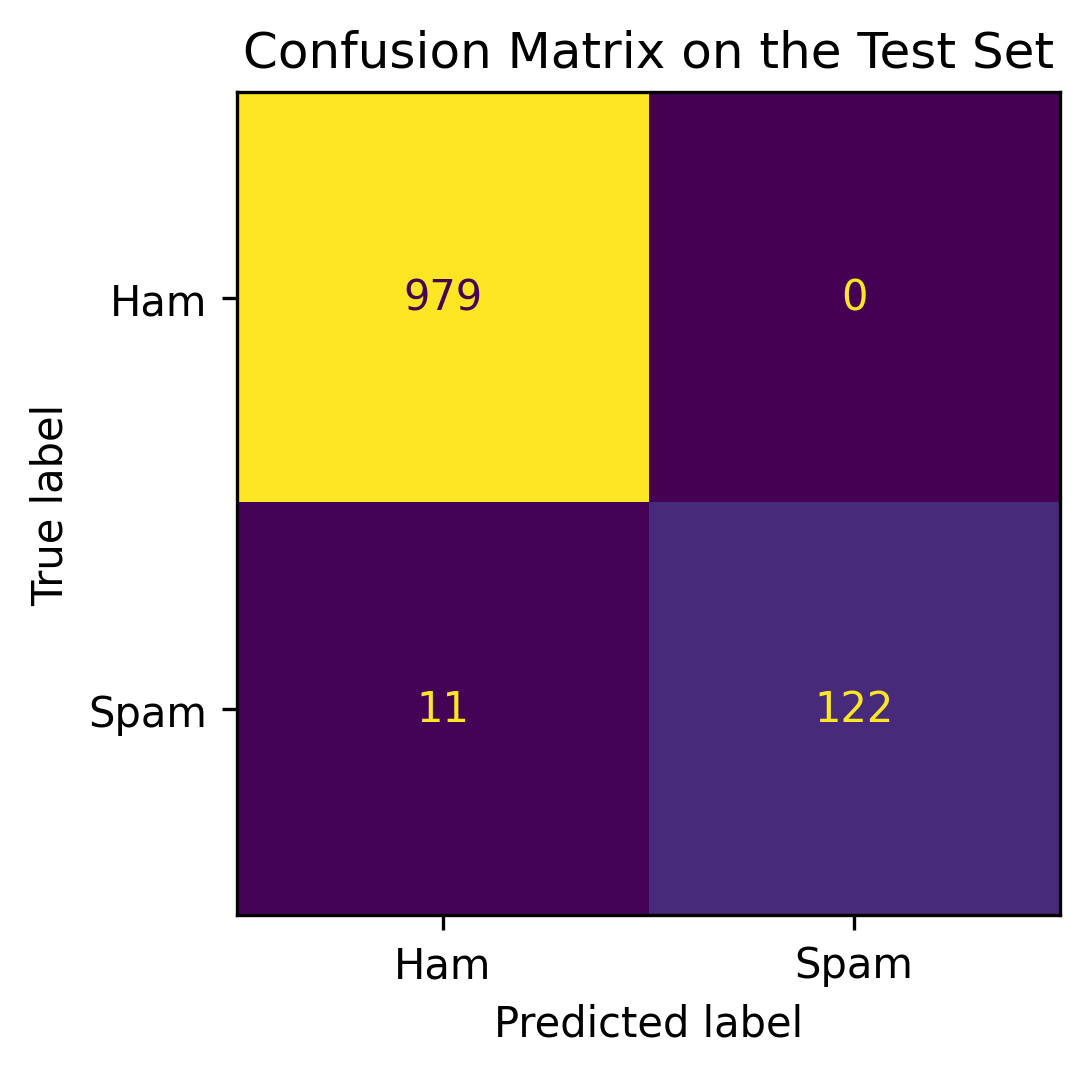
\includegraphics[width=0.82\columnwidth]{figures/confusion_matrix.png}
\caption{Observed test-set confusion matrix. Eleven spam messages are missed, while no ham message is incorrectly labeled as spam.}
\label{fig:cm}
\end{figure}

The matrix contains 979 true negatives, 122 true positives, 11 false negatives, and zero false positives. The corresponding false-negative rate is 8.27\%, meaning that approximately one in twelve spam messages in this test partition is missed. The false-positive rate is 0\% on this specific split.


The operational asymmetry is therefore clear: the system is conservative when assigning the spam label. In the observed test partition it never blocked a ham message, but it failed to identify 11 spam messages.

\subsection{Error-Sensitive Interpretation}
To make the result easier to interpret, Table~\ref{tab:errorprofile} expresses the same confusion matrix through decision-oriented quantities.

\begin{table}[t]
\caption{Error-Sensitive Interpretation of the Observed Confusion Matrix}
\label{tab:errorprofile}
\centering
\scriptsize
\begin{tabular}{p{2.3cm}p{4.1cm}c}
\toprule
Measure & Interpretation & Value \\
\midrule
Specificity & Fraction of ham correctly retained & 100.00\% \\
FPR & Fraction of ham incorrectly marked spam & 0.00\% \\
Recall & Fraction of spam detected & 91.73\% \\
FNR & Fraction of spam missed & 8.27\% \\
NPV & Fraction of predicted ham that is truly ham & 98.89\% \\
Balanced accuracy & Mean of positive and negative recalls & 95.86\% \\
MCC & Correlation-style summary of all four cells & 0.9524 \\
\bottomrule
\end{tabular}
\end{table}

These values produce a more nuanced conclusion than accuracy alone. The model is highly effective on the observed split, but its performance is not symmetric across the two error types. In a user-facing filter, a false negative allows an unwanted message to reach the user, whereas a false positive could hide an important legitimate message. The preferred operating point would therefore depend on the intended application.

\begin{figure}[t]
\centering
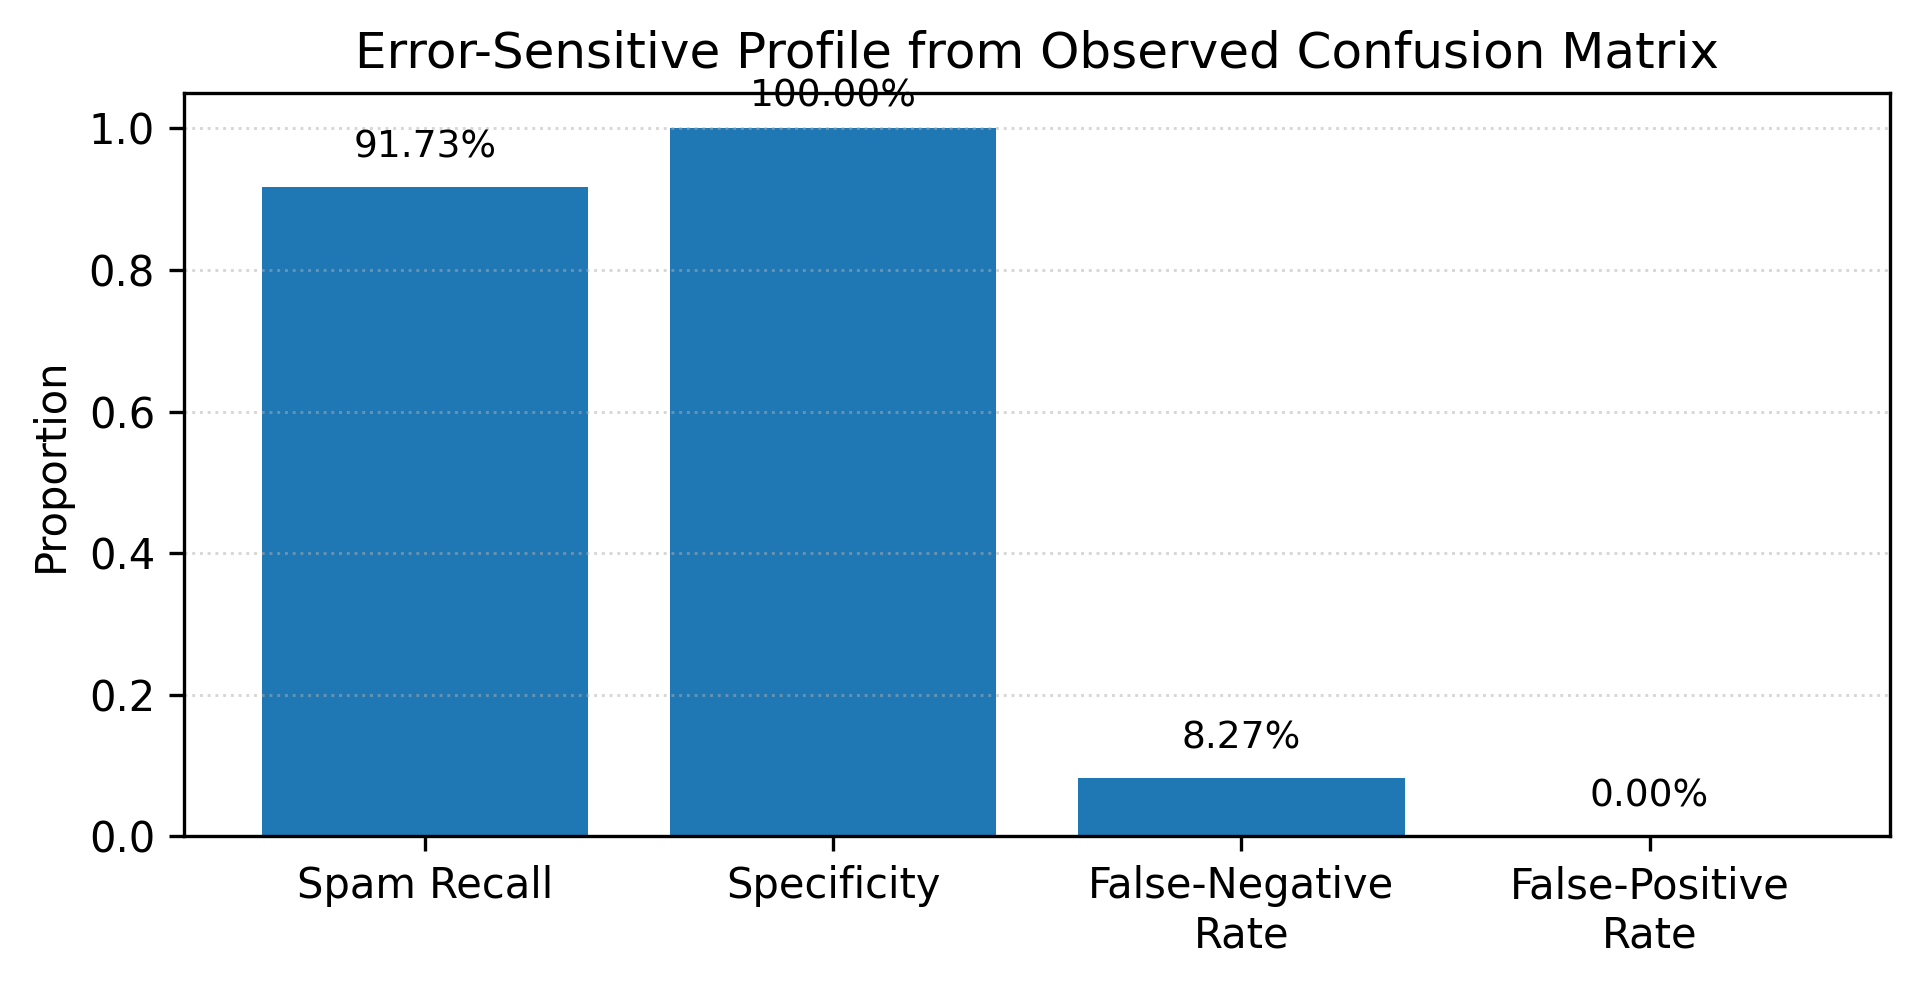
\includegraphics[width=0.96\columnwidth]{figures/error_profile.png}
\caption{Derived error-sensitive profile from the observed confusion matrix. The values emphasize the asymmetry between missed spam and incorrectly flagged ham.}
\label{fig:errorprofile}
\end{figure}

\subsection{Consistency Checks}
The reported metrics can be independently reconstructed from the confusion matrix. Accuracy is $(979+122)/1112=0.9901$. Spam recall is $122/133=0.9173$. Spam precision is $122/(122+0)=1.0$. This internal consistency check is important because the confusion matrix, rather than rounded percentages, preserves the underlying counts.

\section{Discussion}
\subsection{What the Result Does and Does Not Show}
The experiment demonstrates that a standard bag-of-words representation combined with Multinomial Naive Bayes can perform strongly on the supplied SMS corpus. The observed 99.01\% accuracy and 95.69\% spam F1-score indicate that the baseline captures substantial lexical regularities in the data.

The result is consistent with the broader body of work on classical text classification and SMS filtering~\cite{sebastiani2002ml,mccallum1998nb,cormack2007feature,almeida2011sms}. It also aligns with the more recent finding that bag-of-words representations can remain competitive in lightweight SMS spam pipelines even when modern comparative studies include many additional feature and classifier combinations~\cite{senol2026pipeline}.

At the same time, the result cannot establish universal superiority over Logistic Regression, Support Vector Machines, character n-grams, semantic normalization, neural networks, or transformer models because those alternatives were not evaluated in this experiment. The paper therefore treats the classifier as a baseline, not as a final optimal solution.

\subsection{Why Error Analysis Matters}
The confusion matrix reveals a potentially important distinction hidden by accuracy. A test accuracy of 99.01\% may appear nearly perfect, but the model still misses 11 of 133 spam messages. In an operational deployment, that residual miss rate may matter more than the aggregate percentage.

This interpretation is especially relevant because the dataset is imbalanced. Prior work has shown that precision-recall analysis can be more informative than ROC-based summaries in such settings~\cite{davis2006pr,saito2015pr}. The present experiment does not produce a full precision-recall curve because the original code records hard predictions rather than decision scores. Nevertheless, class-wise precision, recall, F1, balanced accuracy, and MCC provide more context than accuracy alone.

\subsection{Comparison With Prior Research}
The observed result should not be compared numerically against unrelated papers without accounting for dataset version, preprocessing, split policy, class-balancing method, and classifier configuration. For example, the recent 2026 systematic study evaluates multiple feature representations, feature-selection methods, imbalance strategies, and classifiers, whereas the present work intentionally evaluates only one lightweight pipeline~\cite{senol2026pipeline}.

Similarly, studies that introduce semantic normalization or more sophisticated text processing alter the input representation and therefore do not constitute controlled comparisons with the present experiment~\cite{almeida2016normalization}. The appropriate interpretation is that the current baseline establishes a reproducible reference point for future experiments, not that it settles the SMS spam detection problem.

\subsection{Computational Considerations}
One practical advantage of the pipeline is its small implementation surface. CountVectorizer produces sparse matrices, while Multinomial Naive Bayes uses straightforward parameter estimation. The implementation is therefore appropriate for CPU-only experimentation and lightweight prototypes. However, this study does not quantify the claimed efficiency: no wall-clock training time, inference latency, peak memory, vocabulary size, or model footprint was captured during the original run.

The study does not report training time, memory consumption, or inference throughput because those quantities were not recorded in the supplied experiment. Claiming a specific runtime would therefore be unsupported. A future version should record these quantities directly and evaluate whether small increases in accuracy justify additional computational cost.

\subsection{Deployment Implications}
The observed absence of false positives is operationally attractive but should not be overinterpreted. The number is zero only for one held-out sample. In a changing environment, message distributions shift and attackers can deliberately alter lexical patterns. Spam filtering is therefore an adversarial problem as well as a classification problem~\cite{almeida2012occam}.

A practical deployment could use this classifier as a first-stage lexical filter, followed by a second-stage model for uncertain messages. Such a cascade is outside the current experiment, but it provides a realistic pathway from a small baseline to a more robust architecture.

\subsection{How the Baseline Supports Stronger Comparative Studies}
The current experiment is deliberately single-model, but its configuration can serve as a reference condition for a more rigorous comparative study. Feature-selection research has shown that large reductions in vocabulary can sometimes preserve or even improve text-classification performance, making feature-space analysis a natural extension of the present pipeline~\cite{yang1997feature}. When multiple classifiers are compared, statistical testing should be planned around repeated measurements rather than a single accuracy table; Dem\v{s}ar recommends non-parametric procedures such as the Wilcoxon signed-rank test for paired classifier comparisons across data sets~\cite{demsar2006}. For the current one-dataset study, inferential testing is intentionally not claimed. Instead, the contribution is a reproducible reference configuration against which future feature and classifier variants can be compared under identical data splits.

\begin{table}[t]
\caption{Recommended Extensions for a Follow-Up Comparative Study}
\label{tab:futurecompare}
\centering
\scriptsize
\begin{tabular}{p{2.2cm}p{3.9cm}}
\toprule
Extension & Purpose \\
\midrule
TF--IDF & Test whether term-frequency normalization improves robustness \\
Word $n$-grams & Capture short phrase information absent from unigram counts \\
Character $n$-grams & Test robustness to spelling variation and obfuscation \\
Linear SVM & Compare a strong sparse linear decision boundary \\
Logistic Regression & Compare probabilistic linear classification \\
Repeated stratified CV & Estimate variability across data partitions \\
Feature selection & Measure accuracy--dimensionality trade-offs \\
\bottomrule
\end{tabular}
\end{table}

\section{Threats to Validity}
\subsection{Internal Validity}
The most important internal threat is the use of a single hold-out split without stratification. Because the split was specified in the original experiment, reproducing it exactly is preferable to changing it after observing performance. Nevertheless, repeated stratified cross-validation would provide stronger evidence of model stability.

Another internal threat is the absence of systematic preprocessing analysis. CountVectorizer is used with its default tokenization settings. Alternate token patterns, stop-word policies, stemming, or character features could change the result substantially.

\subsection{External Validity}
The corpus is a benchmark rather than a representation of every modern messaging environment. Newer scam messages may contain different URLs, emojis, multilingual text, shortened links, or social-engineering patterns. The model should therefore not be assumed to generalize automatically to current traffic.

\subsection{Construct Validity}
The label is interpreted as spam versus ham because that is how the dataset is annotated. However, real-world operational categories such as marketing, fraud, phishing, and ordinary commercial messages may have different meanings and costs. A deployment would need a task definition aligned with the actual harm it is trying to prevent.

\subsection{Reproducibility Validity}
The distinction between the 5,559-row local file and the 5,574-instance public record creates a subtle reproducibility issue. The present paper addresses it explicitly. A future release should also archive the exact CSV version, preprocessing script, Python package versions, and system configuration.

\section{Benchmark Extension Protocol}
To convert the present single-model study into a stronger comparative paper, a controlled benchmark should preserve the same dataset provenance while varying one modeling factor at a time. The recommended benchmark compares the current word-count Multinomial Naive Bayes baseline with TF--IDF+Naive Bayes, word 1--2 grams, character 3--5 grams, Logistic Regression, and Linear SVM. The accompanying benchmark script implements this protocol with leakage-safe pipelines and repeated stratified folds; the resulting comparative numbers are intentionally not reported here because the exact local CSV used for the original 5,559-row experiment was not available in the current artifact set. These are therefore execution-ready planned experiments, not claimed results.


For the comparative study, the preferred protocol is repeated stratified $5$-fold cross-validation, reporting mean $\pm$ standard deviation for accuracy, precision, recall, F1, balanced accuracy, and MCC. Cross-validation is widely used to estimate predictive performance and can be preferable to a single hold-out split when the goal is comparative model assessment~\cite{kohavi1995cv,varma2006cv}.

\section{Future Work}
The proposed baseline provides a starting point for several extensions.

First, the same corpus should be evaluated with controlled representation baselines, including CountVectorizer, TF--IDF, word bigrams, and character $n$-grams. The current manuscript does not present these alternatives as completed experiments. This would convert the current single-model study into a controlled feature-representation experiment.

Second, alternative classifiers such as Logistic Regression, Linear SVM, and complement-style Naive Bayes variants should be evaluated under identical conditions. Joachims' work on high-dimensional text classification provides a classical justification for including linear margin-based methods in such a comparison~\cite{joachims1998svm}.

Third, repeated stratified cross-validation should replace the single hold-out split for the comparative study, with mean $\pm$ standard deviation reported for the principal metrics. The single split should then be retained only as the exact reproducibility experiment reported here.

Fourth, the 11 false-negative messages should be manually categorized. Categories could include shortened or obfuscated URLs, conversationally phrased spam, unusual tokenization, multilingual text, and messages that resemble ordinary personal communication. This would connect the quantitative result to interpretable error mechanisms.

Fifth, a newer SMS or smishing dataset could be used to measure temporal and domain shift. Recent surveys emphasize that the problem is evolving from conventional promotional spam toward more security-relevant smishing patterns~\cite{saidat2024survey}.

Finally, a genuinely resource-aware study should record training time, vocabulary size, memory use, inference latency, and software/hardware configuration. The present paper intentionally does not claim these quantities because they were not captured in the supplied run. This would allow predictive performance to be compared against actual computational cost rather than assuming that classical models are always cheaper.

\section{Conclusion}
This paper presented and evaluated an error-sensitive and reproducible SMS spam detection baseline using CountVectorizer and Multinomial Naive Bayes. On the supplied 5,559-message dataset, the method achieved 99.01\% test accuracy, 100.00\% spam precision, 91.73\% spam recall, and 95.69\% spam F1-score. The confusion matrix contained 979 true negatives, 122 true positives, 11 false negatives, and zero false positives. Derived analysis yielded 95.86\% balanced accuracy, an 8.27\% false-negative rate, and an MCC of 0.9524.

The central contribution is intentionally modest. Rather than proposing a new classifier, the study demonstrates a reproducible and error-sensitive evaluation pattern for a lightweight NLP system and defines a controlled benchmark protocol for future comparative experiments. By explicitly recording dataset provenance, preserving the train/test boundary, reporting class-wise metrics, and analyzing the confusion matrix, the paper provides more information than a single accuracy value while keeping the implementation simple.

The observed performance supports the use of classical sparse text classification as a useful baseline for student research and lightweight prototypes. It does not establish state-of-the-art performance or universal generalization. A stronger next step is a controlled multi-model comparison with repeated validation, explicit resource measurements, and analysis of false-negative message types.

\section*{Acknowledgment}
The authors thank the maintainers of the UCI Machine Learning Repository and the original SMS Spam Collection contributors for making a public benchmark available for research and education.

\balance
\begin{thebibliography}{00}

\bibitem{sebastiani2002ml}
F. Sebastiani, ``Machine learning in automated text categorization,'' \emph{ACM Computing Surveys}, vol. 34, no. 1, pp. 1--47, 2002, doi: 10.1145/505282.505283.

\bibitem{salton1988term}
G. Salton and C. Buckley, ``Term-weighting approaches in automatic text retrieval,'' \emph{Information Processing \& Management}, vol. 24, no. 5, pp. 513--523, 1988, doi: 10.1016/0306-4573(88)90021-0.

\bibitem{mccallum1998nb}
A. McCallum and K. Nigam, ``A comparison of event models for Naive Bayes text classification,'' in \emph{Proc. AAAI-98 Workshop on Learning for Text Categorization}, 1998, pp. 41--48.

\bibitem{androutsopoulos2000spam}
I. Androutsopoulos, G. Paliouras, V. Karkaletsis, G. Sakkis, C. D. Spyropoulos, and P. Stamatopoulos, ``Learning to filter spam e-mail: A comparison of a naive Bayesian and a memory-based approach,'' in \emph{Proc. 4th European Conf. Principles of Data Mining and Knowledge Discovery}, 2000, pp. 1--13.

\bibitem{cormack2007feature}
G. V. Cormack, J. M. G{\'o}mez Hidalgo, and E. Puertas Sanz, ``Feature engineering for mobile (SMS) spam filtering,'' in \emph{Proc. 30th Annual Int. ACM SIGIR Conf. Research and Development in Information Retrieval}, 2007, pp. 871--872, doi: 10.1145/1277741.1277951.

\bibitem{cormack2007spam}
G. V. Cormack, J. M. G{\'o}mez Hidalgo, and E. Puertas Sanz, ``Spam filtering for short messages,'' in \emph{Proc. 16th ACM Conf. Information and Knowledge Management}, 2007, pp. 313--320, doi: 10.1145/1321440.1321486.

\bibitem{almeida2011sms}
T. A. Almeida, J. M. G. Hidalgo, and A. Yamakami, ``Contributions to the study of SMS spam filtering: New collection and results,'' in \emph{Proc. 11th ACM Symposium on Document Engineering}, 2011, pp. 259--262, doi: 10.1145/2034691.2034742.

\bibitem{uci_sms}
T. Almeida and J. Hidalgo, ``SMS Spam Collection,'' UCI Machine Learning Repository, Dataset 228, 2011, doi: 10.24432/C5CC84.

\bibitem{almeida2011dim}
T. A. Almeida, J. Almeida, and A. Yamakami, ``Spam filtering: How the dimensionality reduction affects the accuracy of Naive Bayes classifiers,'' \emph{Journal of Internet Services and Applications}, vol. 1, no. 3, pp. 183--200, 2011, doi: 10.1007/s13174-010-0014-7.

\bibitem{almeida2016normalization}
T. A. Almeida, T. P. Silva, I. Santos, and J. M. G. Hidalgo, ``Text normalization and semantic indexing to enhance instant messaging and SMS spam filtering,'' \emph{Knowledge-Based Systems}, vol. 108, pp. 25--32, 2016, doi: 10.1016/j.knosys.2016.05.001.

\bibitem{almeida2012occam}
T. A. Almeida and A. Yamakami, ``Occam's razor-based spam filter,'' \emph{Journal of Internet Services and Applications}, vol. 3, pp. 245--253, 2012, doi: 10.1007/s13174-012-0067-x.

\bibitem{joachims1998svm}
T. Joachims, ``Text categorization with support vector machines: Learning with many relevant features,'' in \emph{Proc. European Conf. Machine Learning}, 1998, pp. 137--142, doi: 10.1007/BFB0026683.

\bibitem{pedregosa2011sklearn}
F. Pedregosa, G. Varoquaux, A. Gramfort, V. Michel, B. Thirion, O. Grisel, M. Blondel, P. Prettenhofer, R. Weiss, V. Dubourg, J. Vanderplas, A. Passos, D. Cournapeau, M. Brucher, M. Perrot, and E. Duchesnay, ``Scikit-learn: Machine learning in Python,'' \emph{Journal of Machine Learning Research}, vol. 12, pp. 2825--2830, 2011.

\bibitem{davis2006pr}
J. Davis and M. Goadrich, ``The relationship between precision-recall and ROC curves,'' in \emph{Proc. 23rd Int. Conf. Machine Learning}, 2006, pp. 233--240, doi: 10.1145/1143844.1143874.

\bibitem{saito2015pr}
T. Saito and M. Rehmsmeier, ``The precision-recall plot is more informative than the ROC plot when evaluating binary classifiers on imbalanced datasets,'' \emph{PLoS ONE}, vol. 10, no. 3, p. e0118432, 2015, doi: 10.1371/journal.pone.0118432.

\bibitem{saidat2024survey}
M. R. Al Saidat, S. Y. Yerima, and K. Shaalan, ``Advancements of SMS spam detection: A comprehensive survey of NLP and ML techniques,'' \emph{Procedia Computer Science}, vol. 244, pp. 248--259, 2024, doi: 10.1016/j.procs.2024.10.198.

\bibitem{senol2026pipeline}
T. Senol, H. Takci, and A. Seker, ``SMS spam detection via a systematic machine learning pipeline: Feature engineering, hyperparameter optimizing, scaling, and ensemble learning,'' \emph{Journal of Engineering Research}, 2026, doi: 10.1016/j.jer.2026.05.020.



\bibitem{delany2012methods}
S. J. Delany, M. Buckley, and D. Greene, ``SMS spam filtering: Methods and data,'' \emph{Expert Systems with Applications}, vol. 39, no. 10, pp. 9899--9908, 2012, doi: 10.1016/j.eswa.2012.02.053.

\bibitem{gomez2006content}
J. M. G. Hidalgo, G. C. Bringas, E. P. Sanz, and F. C. Garcia, ``Content based SMS spam filtering,'' in \emph{Proc. 2006 ACM Symposium on Document Engineering}, 2006, doi: 10.1145/1166160.1166191.

\bibitem{yang1997feature}
Y. Yang and J. O. Pedersen, ``A comparative study on feature selection in text categorization,'' in \emph{Proc. 14th Int. Conf. Machine Learning}, 1997, pp. 412--420.

\bibitem{agresti1998ci}
A. Agresti and B. A. Coull, ``Approximate is better than `exact' for interval estimation of binomial proportions,'' \emph{The American Statistician}, vol. 52, no. 2, pp. 119--126, 1998, doi: 10.1080/00031305.1998.10480550.

\bibitem{demsar2006}
J. Dem\v{s}ar, ``Statistical comparisons of classifiers over multiple data sets,'' \emph{Journal of Machine Learning Research}, vol. 7, pp. 1--30, 2006.


\bibitem{chicco2020mcc}
D. Chicco and G. Jurman, ``The advantages of the Matthews correlation coefficient (MCC) over F1 score and accuracy in binary classification evaluation,'' \emph{BMC Genomics}, vol. 21, art. no. 6, 2020, doi: 10.1186/s12864-019-6413-7.

\bibitem{kohavi1995cv}
R. Kohavi, ``A study of cross-validation and bootstrap for accuracy estimation and model selection,'' in \emph{Proc. 14th Int. Joint Conf. Artificial Intelligence}, 1995, pp. 1137--1145.

\bibitem{varma2006cv}
S. Varma and R. Simon, ``Bias in error estimation when using cross-validation for model selection,'' \emph{BMC Bioinformatics}, vol. 7, art. no. 91, 2006, doi: 10.1186/1471-2105-7-91.

\end{thebibliography}

\end{document}
